\everymath{\displaystyle}
%\documentclass[pdftex,a4paper]{article}
\documentclass[a4paper]{article}
%%classes: article, report, book, proc, amsproc

%%%%%%%%%%%%%%%%%%%%%%%%
%% Misc
% para acertar os acentos
\usepackage[brazilian]{babel}
%\usepackage[portuguese]{babel}
% \usepackage[english]{babel}
% \usepackage[T1]{fontenc}
% \usepackage[latin1]{inputenc}
\usepackage[utf8]{inputenc}
\usepackage{indentfirst}
\usepackage{fullpage}
% \usepackage{graphicx} %See PDF section
\usepackage{multicol}
\setlength{\columnseprule}{0.5pt}
\setlength{\columnsep}{20pt}
%%%%%%%%%%%%%%%%%%%%%%%%
%%%%%%%%%%%%%%%%%%%%%%%%
%% PDF support

\usepackage[pdftex]{color,graphicx}
% %% Hyper-refs
\usepackage[pdftex]{hyperref} % for printing
% \usepackage[pdftex,bookmarks,colorlinks]{hyperref} % for screen

%% \newif\ifPDF
%% \ifx\pdfoutput\undefined\PDFfalse
%% \else\ifnum\pdfoutput > 0\PDFtrue
%%      \else\PDFfalse
%%      \fi
%% \fi

%% \ifPDF
%%   \usepackage[T1]{fontenc}
%%   \usepackage{aeguill}
%%   \usepackage[pdftex]{graphicx,color}
%%   \usepackage[pdftex]{hyperref}
%% \else
%%   \usepackage[T1]{fontenc}
%%   \usepackage[dvips]{graphicx}
%%   \usepackage[dvips]{hyperref}
%% \fi

%%%%%%%%%%%%%%%%%%%%%%%%


%%%%%%%%%%%%%%%%%%%%%%%%
%% Math
\usepackage{amsmath,amsfonts,amssymb}
% para usar R de Real do jeito que o povo gosta
\usepackage{amsfonts} % \mathbb
% para usar as letras frescas como L de Espaco das Transf Lineares
% \usepackage{mathrsfs} % \mathscr

% Oferecer seno e tangente em pt, com os comandos usuais.
\providecommand{\sin}{} \renewcommand{\sin}{\hspace{2pt}\mathrm{sen}}
\providecommand{\tan}{} \renewcommand{\tan}{\hspace{2pt}\mathrm{tg}}

% dt of integrals = \ud t
\newcommand{\ud}{\mathrm{\ d}}
%%%%%%%%%%%%%%%%%%%%%%%%

\title{Avaliação Parcial da disciplina de Metodologia Científica}
\date{}
\author{Docente: Felipe Figueiredo\\
  \url{prof.felipefigueiredo@gmail.com}\\
  \url{http://sites.google.com/site/proffelipefigueiredo}
}
\begin{document}
\maketitle
\abstract{Nesta avaliação parcial, os alunos deverão redigir um texto
  dissertativo que simule um projeto de pesquisa. Aqui estão gráficos
  que descrevem um conjunto de dados preliminar, como se obtidos em um
  projeto piloto. Caberá aos alunos (a) formular um problema de
  pesquisa baseado nesses dados preliminares, (b) indicar que outros
  tipos de dados deverão ser coletados para atender às questões
  levantadas, (c) justificar suas escolhas, preferencialmente com
  algumas referências bibliográficas.

  Obs: Os dados preliminares aqui contidos são altamente fictícios,
  portanto não há pergunta ou resposta correta nesta avaliação, apenas
  bons argumentos. Confronte-os com suas expectativas e intuição.}

\newpage

%%%%%%%%%%%%%%%%%%%%%%%%
%% Título e cabeçalho
%\noindent\parbox[c]{.15\textwidth}{
\includegraphics[width=.15\textwidth]{logo}}\hfill
\parbox[c]{.825\textwidth}{\raggedright%
  \sffamily {\LARGE

Metodologia Científica

Avaliação Parcial

\par\bigskip}
{Prof: Felipe Figueiredo\par}
{\url{http://sites.google.com/site/proffelipefigueiredo}\par}
}

Versão: \verb|YYYYMMDD|

%%%%%%%%%%%%%%%%%%%%%%%%


%%%%%%%%%%%%%%%%%%%%%%%%

\section{Objetivos}
O objetivo primário desta avaliação é proporcionar ao discente uma
primeira oportunidade de redigir um anteprojeto, seguindo normas
adequadas à pesquisa científica, e ao programa de Pós-Graduação. Para
tal, serão avaliados a clareza na exposição textual, e a exposição do
material, seguindo os padrões estabelecidos de formatação de página,
parágrafo, referências e demais elementos.

O objetivo secundário desta avaliação é estimular tanto a criatividade
acadêmica como a habilidade de formulação de problemas.


\section{Contexto}

\begin{itemize}
\item objetivo: os alunos devem, já sabendo a resposta por experiência
  própria, elaborar um projeto fictício para testar essa pergunta.
\item premissa: o dataset é um preliminar, de um estudo piloto, que
  servirá de base para o texto.
\item Devem pensar em como formular a hipótese, e descrever os
  resultados preliminares.
\end{itemize}
\section{Problema}

\begin{itemize}
\item existe uma correlação entre a circunferência abdominal e doença
  cardíaca?
\end{itemize}

\begin{figure}[h]
  \centering
  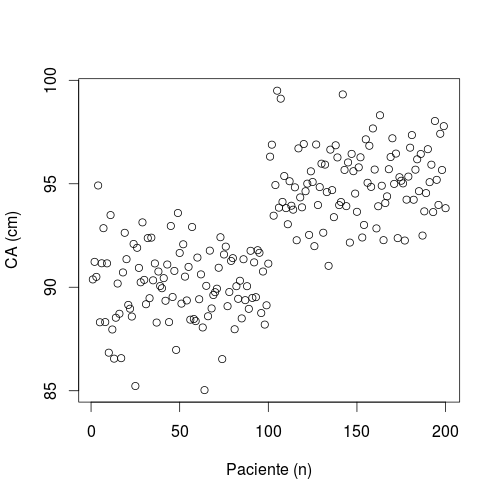
\includegraphics[width=.5\textwidth]{dispersao}
  \caption{Gráfico de dispersão da Circunferência abdominal (CA) de
    cada paciente.}
  \label{fig:dispersao}
\end{figure}

\begin{figure}[h]
  \centering
  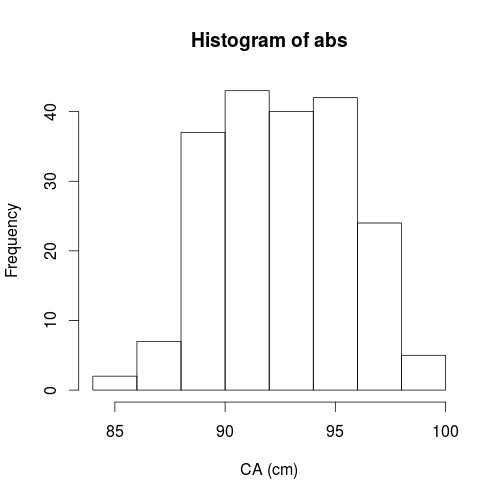
\includegraphics[width=.5\textwidth]{histograma}
  \caption{Histograma de frequências da Circunferência abdominal (CA)
    de homens adultos.}
  \label{fig:histograma}
\end{figure}

\begin{figure}[h]
  \centering
  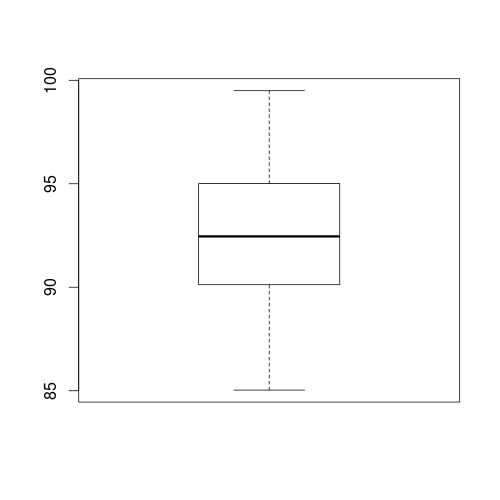
\includegraphics[width=.5\textwidth]{boxplot}
  \caption{Boxplot da Circunferência abdominal (CA) de homens
    adultos.}
  \label{fig:boxplot}
\end{figure}

\end{document}
